% Example results
\subsection{Simulation Outline}
The simulation results are images that were created using a specific interferometer layout and a specific sky model. The sky model that was used for the following results was a sky model with 4 points, each of which having a different brightness, or flux. The sky model can be seen in figure \ref{fig:Sky_model}.
\begin{figure}[H]
    \centering
    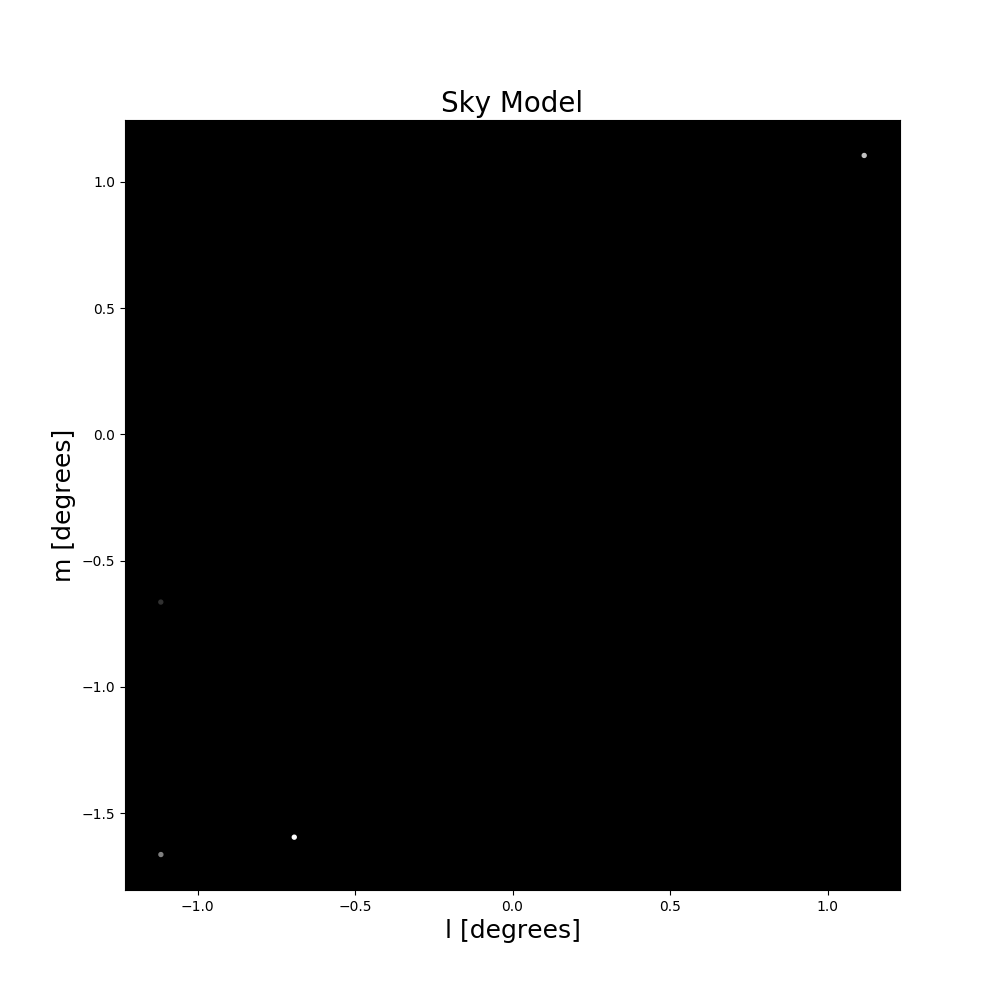
\includegraphics[scale=0.4]{images/4_POINT.png}
    \caption{Sky model for simulation}
    \label{fig:Sky_model}
\end{figure}
\begin{center}
\end{center}
The sky model has a distinctive shape to it, the results from each interferomter should have this shape with a point spread function creating some noise around every point source. \\
Before the results are shown, the point spread functions for KAT-7, HERA-19, which is a real world telescope that we have created a model of for our testing.\cite{HERA-19} and TART will be displayed. These are the interferomters that were used to display the results, the TART interferometer here is a antenna layout that was created from TART's actual layout, it is simple treated here as a tracking array, while in reality it is in fact, not a tracking array, it is a static array that looks in one direction at all times, directly above it.
\begin{figure}[H]
  \centering
  \begin{subfigure}[b]{0.49\textwidth}
    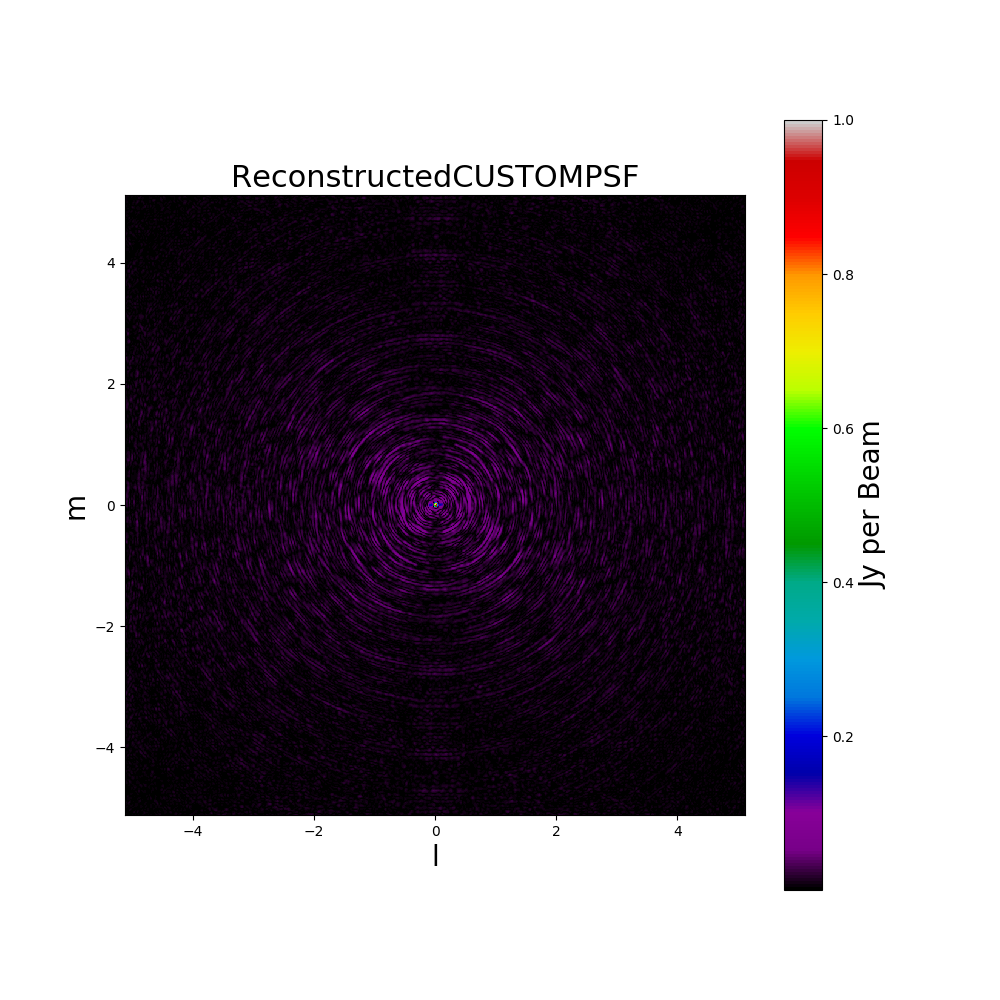
\includegraphics[width=\textwidth]{images/KAT_7_PSF.png}
    \caption{KAT-7 PSF}
    \label{fig:1}
  \end{subfigure}
  %
  \begin{subfigure}[b]{0.49\textwidth}
    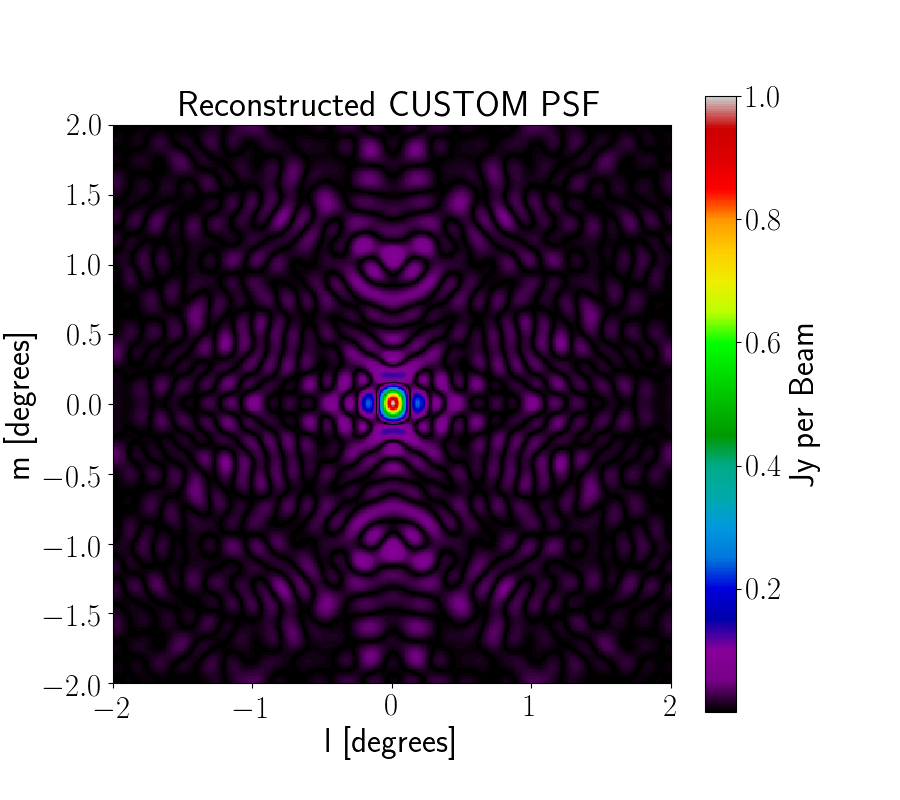
\includegraphics[width=\textwidth]{images/HERA_19_PSF.png}
    \caption{HERA-19 PSF}
    \label{fig:HERA-19 PSF}
  \end{subfigure}
  %
  \newline
  \begin{subfigure}[b]{0.49\textwidth}
    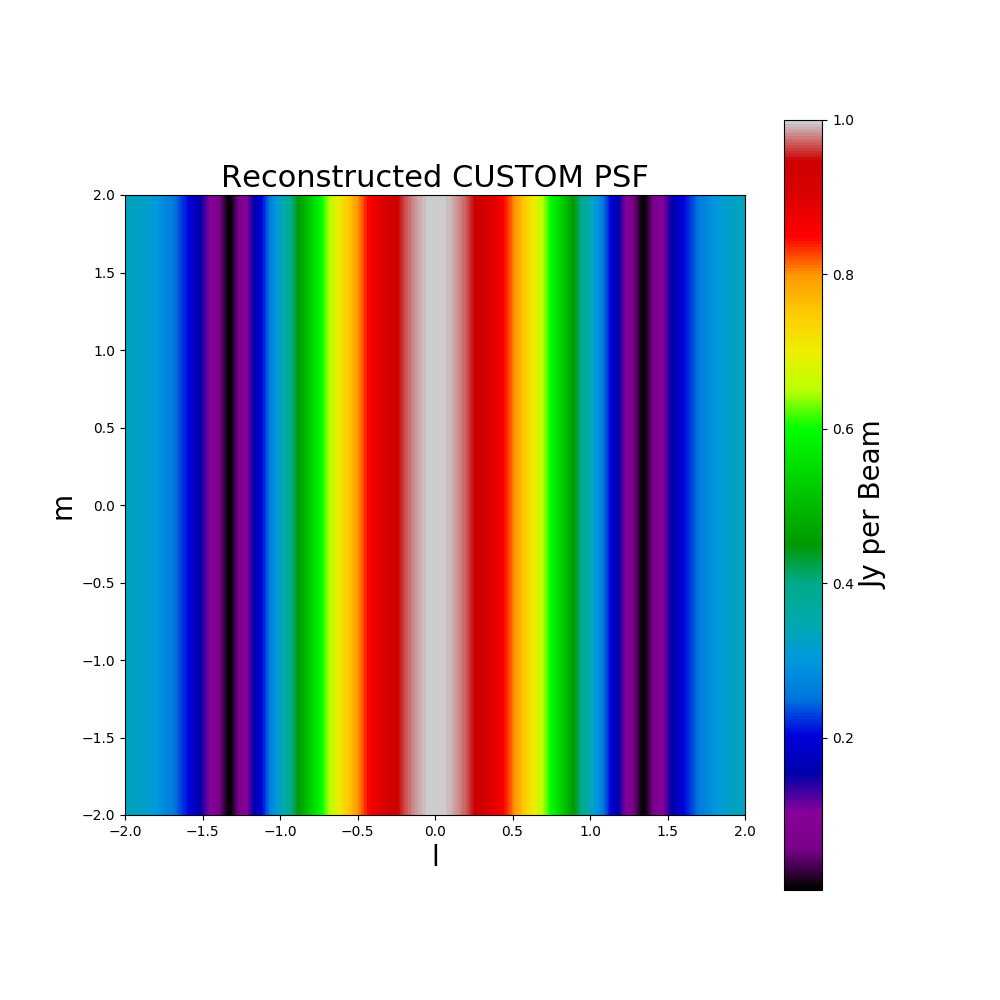
\includegraphics[width=\textwidth]{images/TART_PSF.png}
    \caption{TART PSF}
    \label{fig:TART PSF}
  \end{subfigure}
  %
  \begin{subfigure}[b]{0.49\textwidth}
    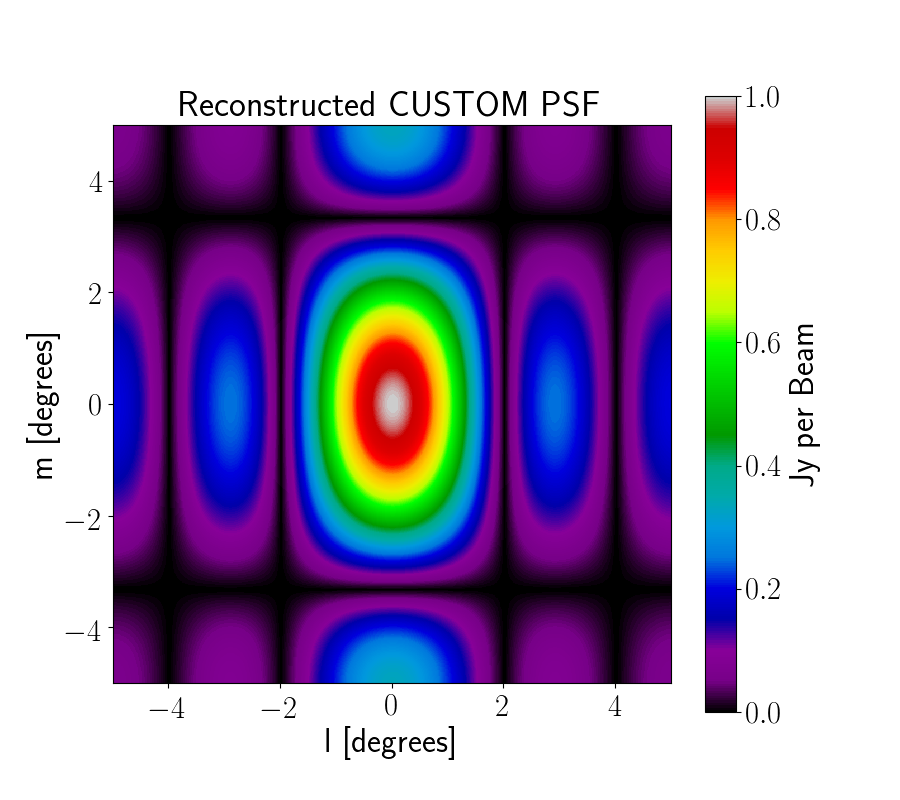
\includegraphics[width=\textwidth]{images/TART_PSF_CORRECT.png}
    \caption{TART PSF \\with larger field of view}
    \label{fig:TART PSF FOV}
    \vspace{-4mm}
  \end{subfigure}
  \caption{Interferometer PSF's}
\end{figure}

\subsection{Simulation Results}
\begin{figure}[H]
  \centering
  \begin{subfigure}[b]{0.49\textwidth}
    \centering
    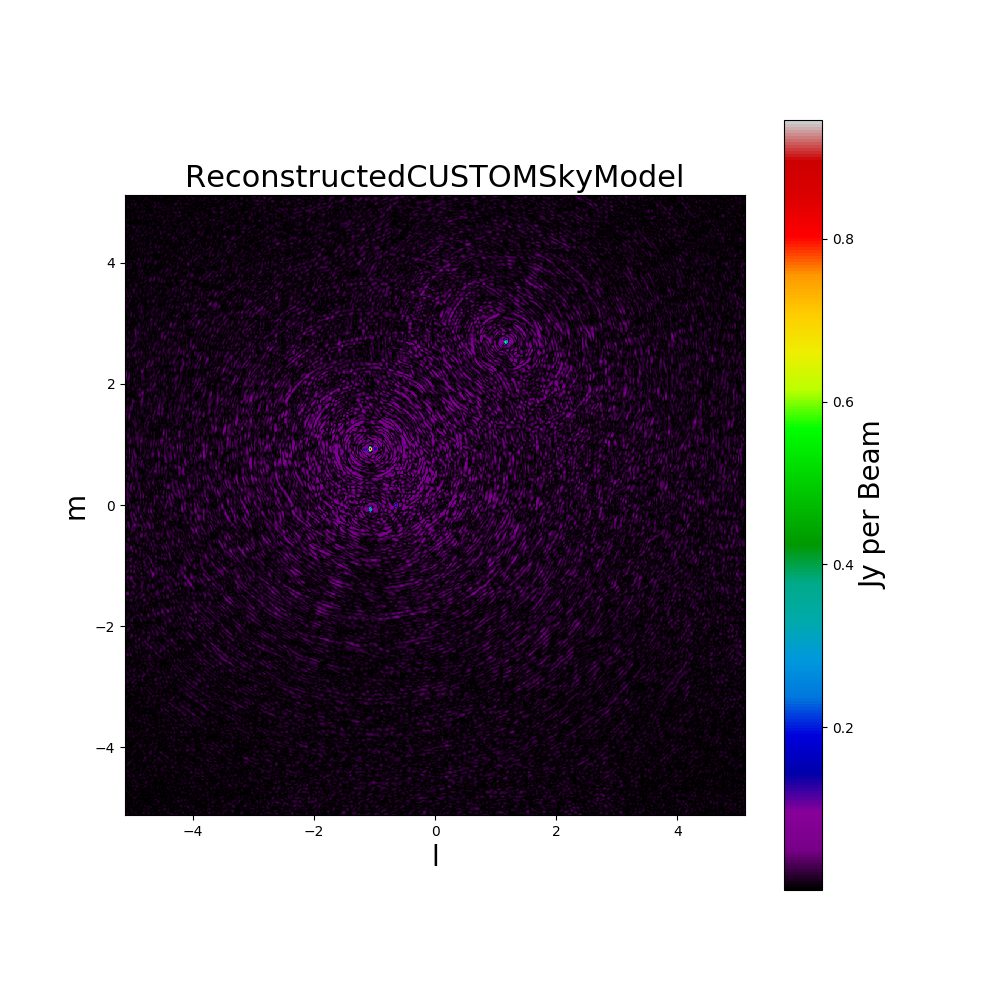
\includegraphics[scale=0.3]{images/RECON_KAT_7_4_POINT.png}
    \caption{A reconstruction from KAT-7 for this sky model using a cell size of $0.01^\circ$ and a 
    field of view of $4^\circ$.}
    \label{fig:kat-7_recon}
  \end{subfigure}
  %
  \begin{subfigure}[b]{0.49\textwidth}
    \centering
    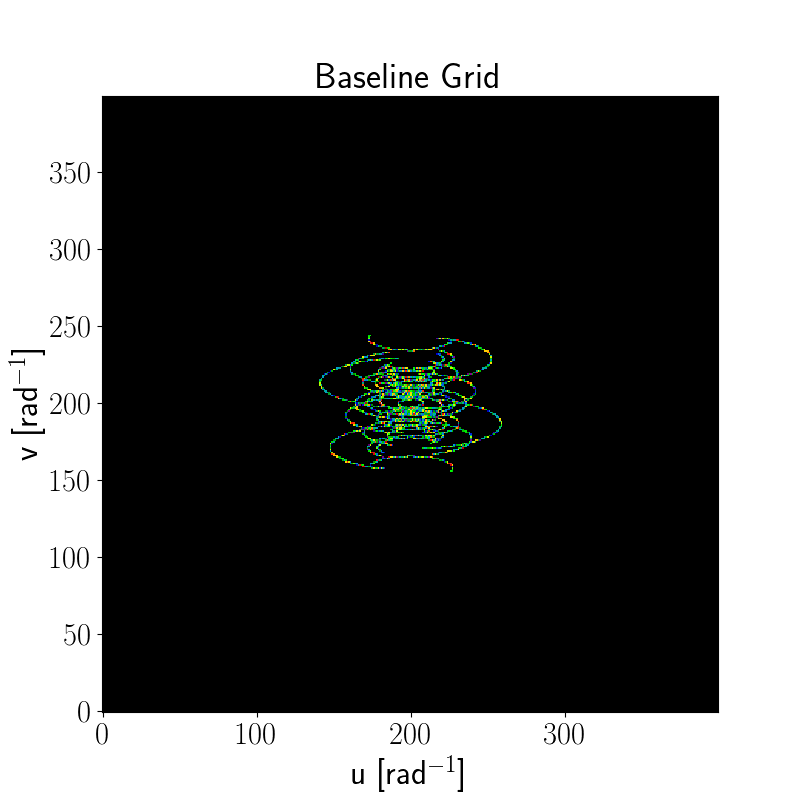
\includegraphics[scale=0.3]{images/KAT_7_4_POINT_GRID.png}
    \caption{The UV grid from KAT-7 for this sky model using a cell size of $0.01^\circ$ and a 
    field of view of $4^\circ$.}
    \label{fig:kat-7_recon_grid}
  \end{subfigure}
  \caption{KAT-7 sky model and grid.}
  \label{fig:kat-7}
 \end{figure}

In figure \ref{fig:kat-7_recon} it can be seen that the brighter sources are easily visible, but the one source that was not as bright is not nearly as visible.  The shape is correct and it can clearly be seen that the point spread function has introduced noise to the image and that it matches the point spread function that was introduced earlier in this section.\\
\begin{figure}[H]
  \centering
  \begin{subfigure}[b]{0.49\textwidth}
    \centering
    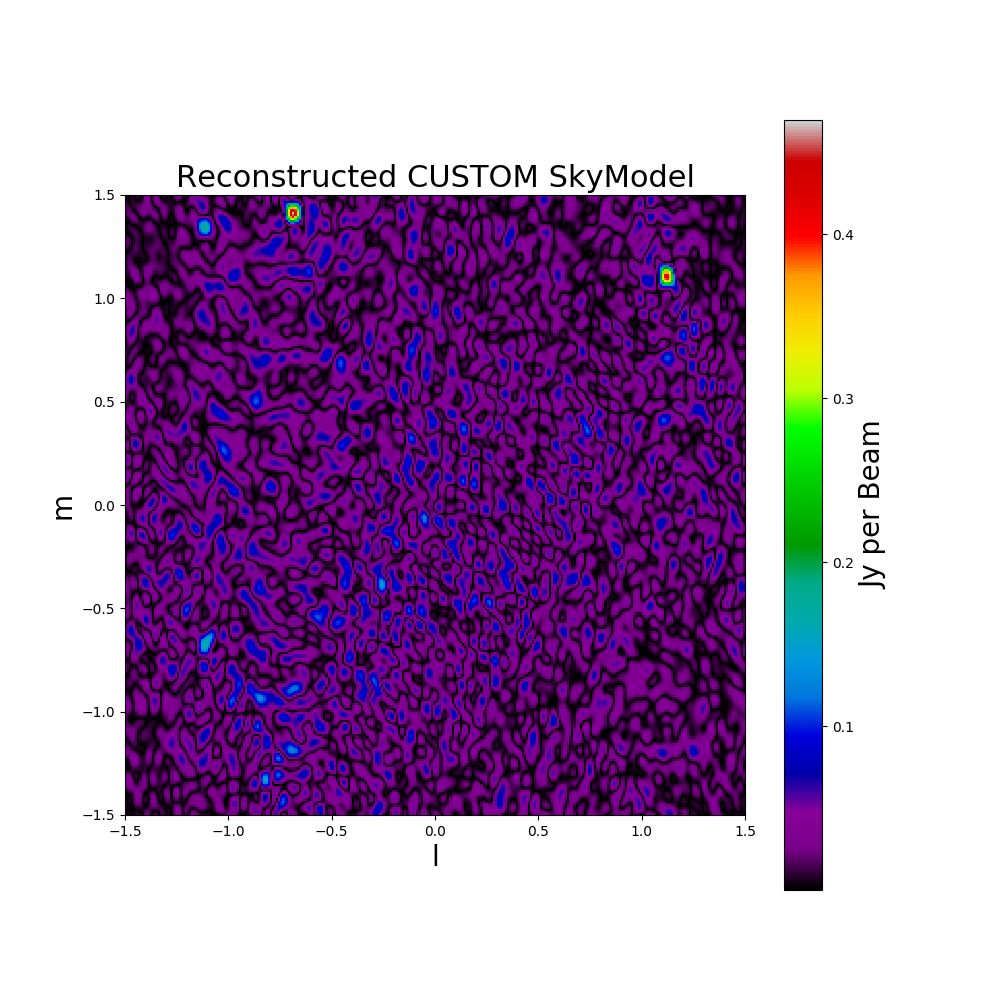
\includegraphics[scale=0.3]{images/RECON_KAT_7_4_POINT_ALIASING.png}
    \caption{A reconstruction from KAT-7 for this sky model using a cell size of $0.01^\circ$ and a field of view of $3^\circ$.}
    \label{fig:kat-7_recon_alias}
  \end{subfigure}
  %
  \begin{subfigure}[b]{0.49\textwidth}
    \centering
    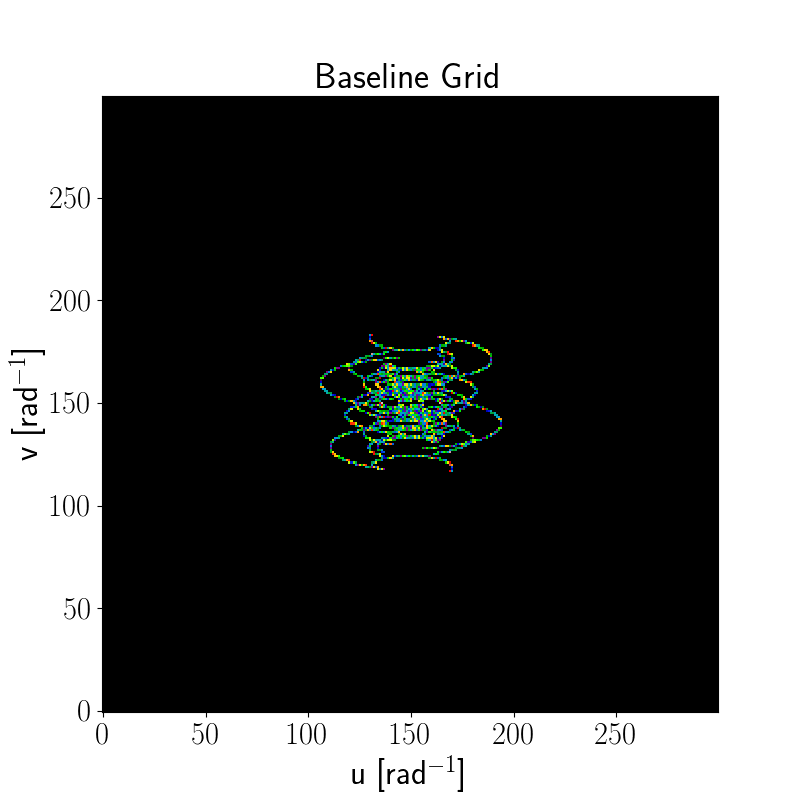
\includegraphics[scale=0.3]{images/KAT_7_4_POINT_GRID_ALIASING.png}
    \caption{The UV grid from KAT-7 for this sky model using a cell size of $0.01^\circ$ and a field of view of $3^\circ$.}
    \label{fig:kat-7_grid_alias}
  \end{subfigure}
  \caption{KAT-7 sky model and grid with aliasing.}
  \label{fig:kat-7_alias}
 \end{figure}

In figure \ref{fig:kat-7_recon_alias} the two sources at the top appear to be in the wrong location, this is due to aliasing as the field of view was not correctly selected. It is important to remember to adhere to the Nyquist Theorem that is outlined in section 2.4.1.

\begin{figure}[H]
  \centering
  \begin{subfigure}[b]{0.49\textwidth}
    \centering
    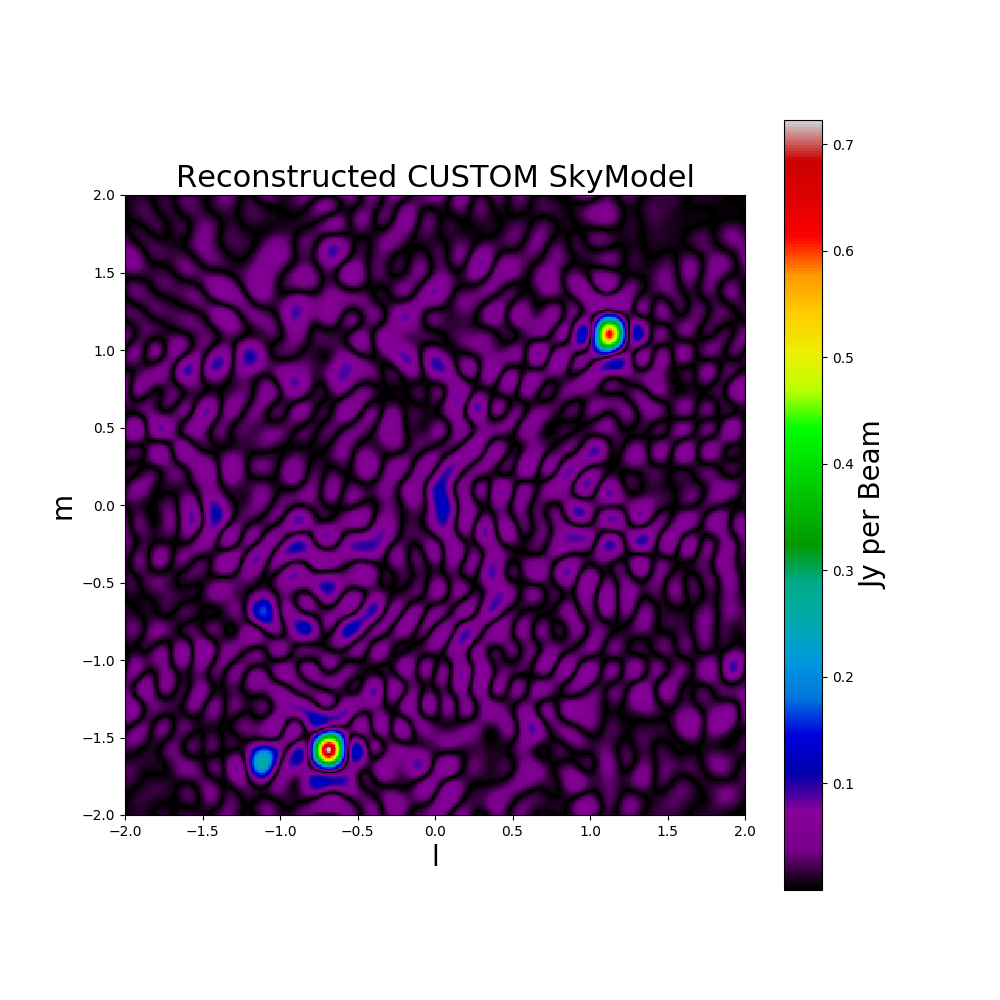
\includegraphics[scale=0.3]{images/RECON_HERA_19_4_POINT.png}
    \caption{A reconstruction from HERA-19 for the sky model using a cell size of $0.01^\circ$ and a field of view of $4^\circ$.}
    \label{fig:hera-19_recon}
  \end{subfigure}
  %
  \begin{subfigure}[b]{0.49\textwidth}
    \centering
    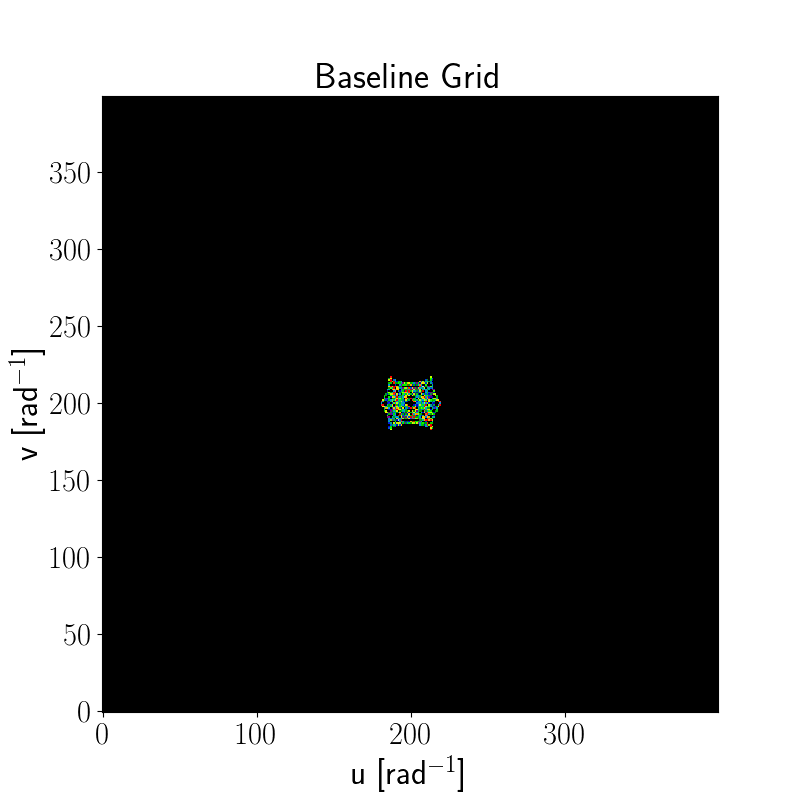
\includegraphics[scale=0.3]{images/HERA_19_4_POINT_GRID.png}
    \caption{The UV grid from HERA-19 for this sky model using a cell size of $0.01^\circ$ and a field of view of $4^\circ$.}
    \label{fig:hera-19_grid}
  \end{subfigure}
  \caption{HERA-19 sky model and grid.}
  \label{fig:HERA-19_model}
 \end{figure}


As with the KAT 7 image, in figure \ref{fig:hera-19_recon} the bright sources are easily visible while the one less bright source is hard to identify. The point spread function has introduced noise to the image around the sources and it is clear that it is the same point spread function that was shown earlier in this section.

\begin{figure}[H]
  \centering
  \begin{subfigure}[b]{0.49\textwidth}
    \centering
    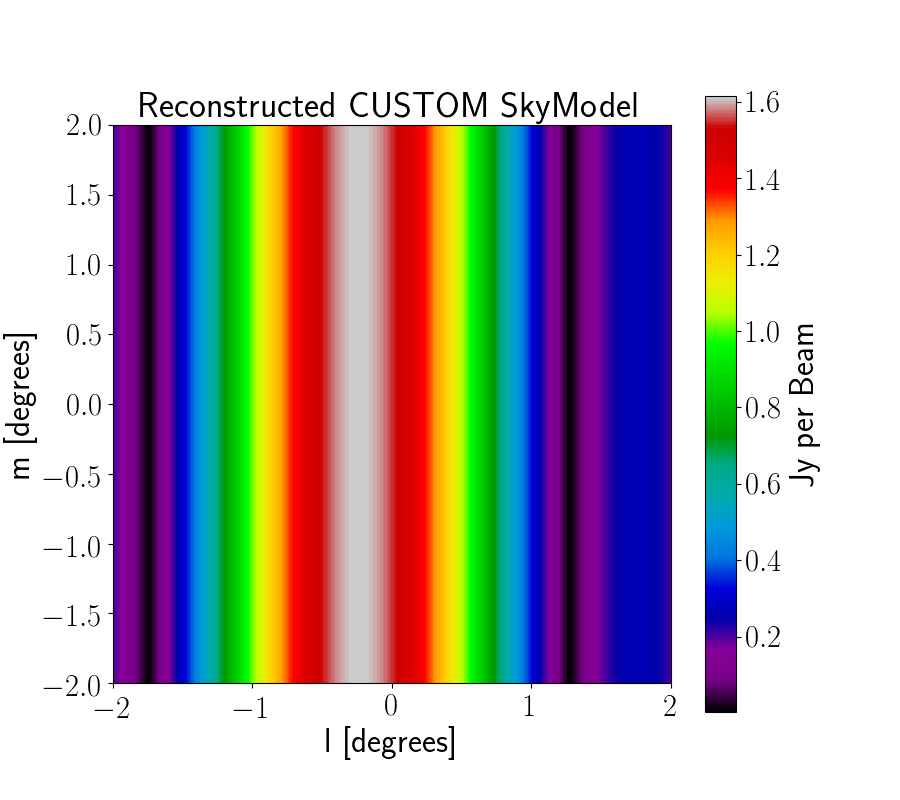
\includegraphics[scale=0.3]{images/RECON_TART_4_POINT.png}
    \caption{A reconstruction from TART for the sky model using a cell size of $0.01^\circ$ and a field of view of $4^\circ$.}
    \label{fig:TART_recon}
  \end{subfigure}
  %
  \begin{subfigure}[b]{0.49\textwidth}
    \centering
    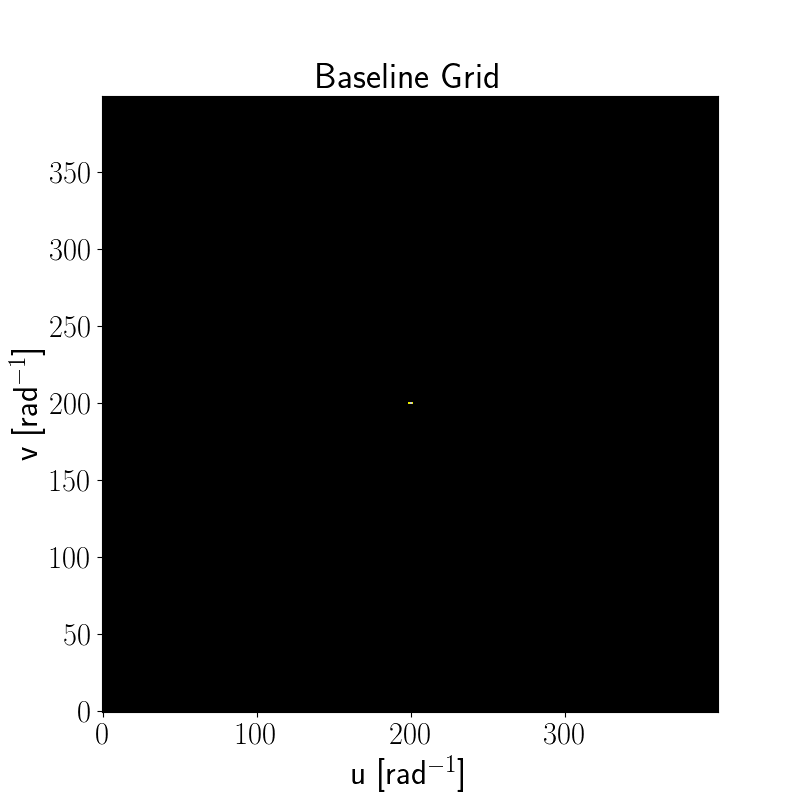
\includegraphics[scale=0.3]{images/TART_4_POINT_GRID.png}
    \caption{The UV grid from TART for this sky model using a cell size of $0.01^\circ$ and a field of view of $4^\circ$.}
    \label{fig:TART_grid}
  \end{subfigure}
  \caption{TART sky model and grid.}
  \label{fig:TART}
 \end{figure}
 
In figure \ref{fig:TART_recon} it is instantly clear that the none of points are at all visible in this reconstruction.

\begin{figure}[H]
  \centering
  \begin{subfigure}[b]{0.49\textwidth}
    \centering
    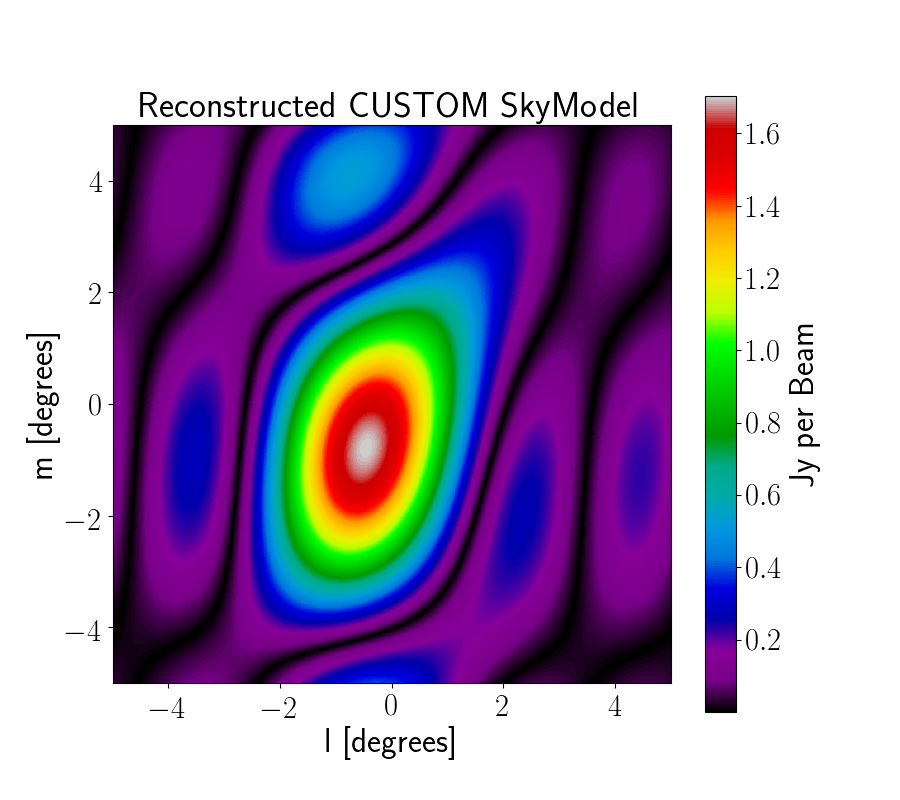
\includegraphics[scale=0.3]{images/RECON_TART_4_POINT_CORRECT.png}
    \caption{A reconstruction from TART for the sky model using a cell size of $0.01^\circ$ and a field of view of $10^\circ$.}
    \label{fig:TART_recon_correct}
  \end{subfigure}
  %
  \begin{subfigure}[b]{0.49\textwidth}
    \centering
    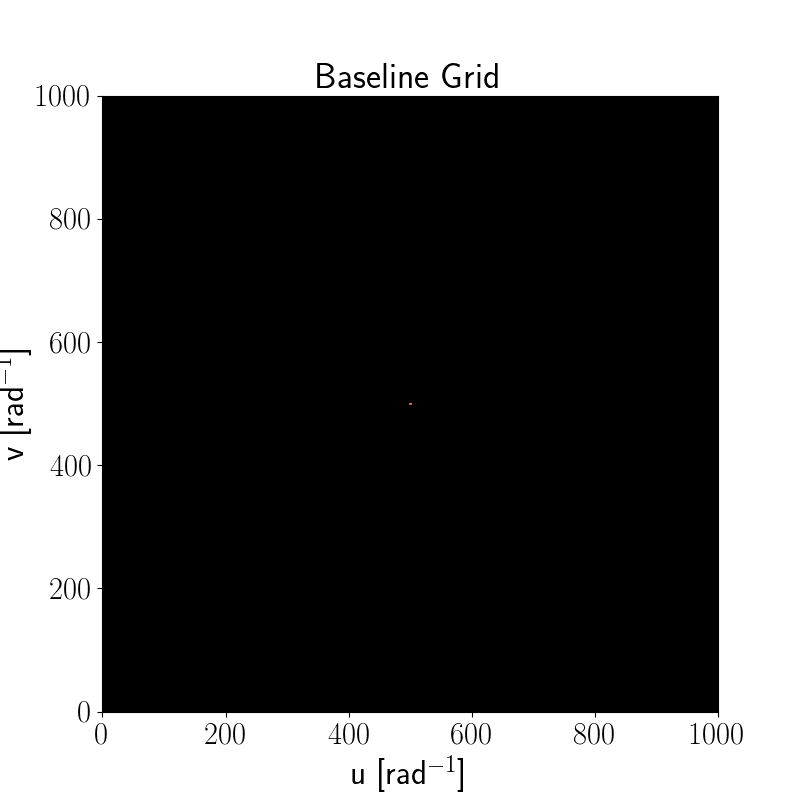
\includegraphics[scale=0.3]{images/TART_4_POINT_GRID_CORRECT.png}
    \caption{The UV grid from TART for this sky model using a cell size of $0.01^\circ$ and a field of view of $10^\circ$.}
    \label{fig:TART_grid_correct}
  \end{subfigure}
  \caption{TART sky model and grid with larger field of view.}
  \label{fig:TART_correct}
 \end{figure}
 
In figure \ref{fig:TART_recon_correct} it is easy to see that the points are not at all visible in this reconstruction, however is is more clear than the example with the smaller field of view, so the TART model does work. The reason for the bad image is because TART is not nearly as powerful as KAT-7 or HERA-19, it is also due to the very small hour angle that was given to TART for this simulation.
It can also be noted that in both images for TART, the color scale is not correct.
\\
\begin{table}[H]
    \centering
    \begin{tabular}{ |p{0.18\textwidth}||p{0.18\textwidth}|p{0.18\textwidth}|p{0.18\textwidth}| p{0.18\textwidth}| }
     \hline
     \multicolumn{5}{|c|}{Simulation Parameters} \\
     \hline
     Interferometer & Hour Angle & Frequency & Cell Size & Field of View \\
     \hline
     KAT-7 & -6 to 6 & 1.4GHz & 0.01 & 4 \\
     HERA-19 & -4 to 4 & 1.4GHz & 0.01 & 4 \\
     TART & -0.6 to 0.6 & 1.5713GHz & 0.01 & 4 \\
     KAT-7 aliasing & -6 to 6 & 1.4GHz & 0.01 & 3 \\
     TART larger field of view & -0.6 to 0.6 & 1.5713GHz & 0.01 & 10 \\
     \hline
    \end{tabular}
    
\end{table}

\subsection{TART Images}
\FloatBarrier
\begin{figure}[H]
  \centering
  \begin{subfigure}[b]{0.49\textwidth}
    \centering
    \includegraphics[scale=0.28]{images/7-11-19_13:41_SA_PIPE_CIRCLES.png}
    \caption{Image from the SA TART interferometer through the pipeline at 13:41 on 7 November 2019.}
    \label{fig:TART_SA}
  \end{subfigure}
  %
  \begin{subfigure}[b]{0.49\textwidth}
    \centering
    \includegraphics[scale=0.35]{images/7-11-19_13:41_SA_WEB_CIRCLES.png}
    \vspace*{6mm}
    \caption{Image from the SA TART interferometer through the API at 13:41 on 7 November 2019.}
    \label{fig:TART_SA_WEB}
  \end{subfigure}
  \caption{Images from the TART pipeline and the web API at 13:41 on 7 November 2019.}
  \label{fig:TART_RESULTS}
\end{figure}
The interferometer can only view the whole sky, the outer circle is the edge of the horizon so everything outside it is noise. This can be seen in figure \ref{fig:TART_SA}. Some points that are easy to identity in both \ref{fig:TART_SA} and \ref{fig:TART_SA_WEB} are circled in red.

\begin{figure}[H]
  \centering
  \begin{subfigure}[b]{0.49\textwidth}
    \centering 
    \includegraphics[scale=0.3]{images/7-11-19_13:41_SA_PIPE_PSF.png}
    \caption{PSF from the SA TART interferometer through the pipeline at 13:41 on 7 November 2019.}
    \label{fig:TART_SA_PSF}
  \end{subfigure}
  %
  \begin{subfigure}[b]{0.49\textwidth}
 \centering
    \includegraphics[scale=0.3]{images/7-11-19_13:41_SA_PIPE_GRID.png}
    \caption{Grid from the SA TART interferometer through the pipeline at 13:41 on 7 November 2019.}
    \label{fig:TART_SA_GRID}
  \end{subfigure}
  \caption{The TART PSF and grid at 13:41 on 7 November 2019.}
  \label{fig:HERA-19}
\end{figure}

The image in figure \ref{fig:TART_SA} and the PSF in figure \ref{fig:TART_SA_PSF} obtained through the pipeline use a cell size of $0.1^\circ$

It is quite clear that the image from the pipeline in figure
\ref{fig:TART_SA} and the image from the TART API in figure \ref{fig:TART_SA_WEB} are similar, there are some points on the pipeline image that are brighter than the points in the API image but others that seem to match perfectly. This is likely due to the color scale being different for both imaging pipelines.
\FloatBarrier
\subsection{Conclusion}
The pipeline works correctly if the correct field of view is chosen for the images and if the user selects the correct cell size.\\
The images obtained from TART in the simulation do not show much detail as TART is not a very powerful interferometer and has a field of view of only 4$^\circ$.
TART is also a whole sky interferometer, this also means that the images are less detailed as they don't focus on a small area of the sky which would allow for higher details. Due to this, TART images will never show high levels of detail. 
As such, the results that are obtained from it will never match what is being produced by more powerful interferometers which focus on specific small fields of view. 
\\The fact that the API and pipeline images are the same shows that the pipeline is working as intended and the project was a success.
% It is however a perfect tool to teach students how radio interferometry works and if this pipeline was turned into a teaching tool it could explain the subject matter while having a real interferometer to show results with.

% Show simulation
%  Image from TART as final result